\chapter{Why Learn AWS?}
AWS are the market leaders in cloud. They are at the forefront of cloud revolution.
AWS has a partner program:

\section{AWS Partner Programs}
3 different tiers:
\begin{enumerate}
	\item select.
	\item advanced.
	\item premier.
\end{enumerate}

types of certificates:
\begin{enumerate}
	\item Practitioner.
	\item Associate.
	\item Professional/Speciality Certificates.
\end{enumerate}

Getting an AWS certificates increases your demand because companies need certain number of certified employees to have access to AWS partner programs/premium lounges etc. These are shown in the figure (\ref{AWS-partner-tiers}).

\begin{figure}[htbp]
	\centering
	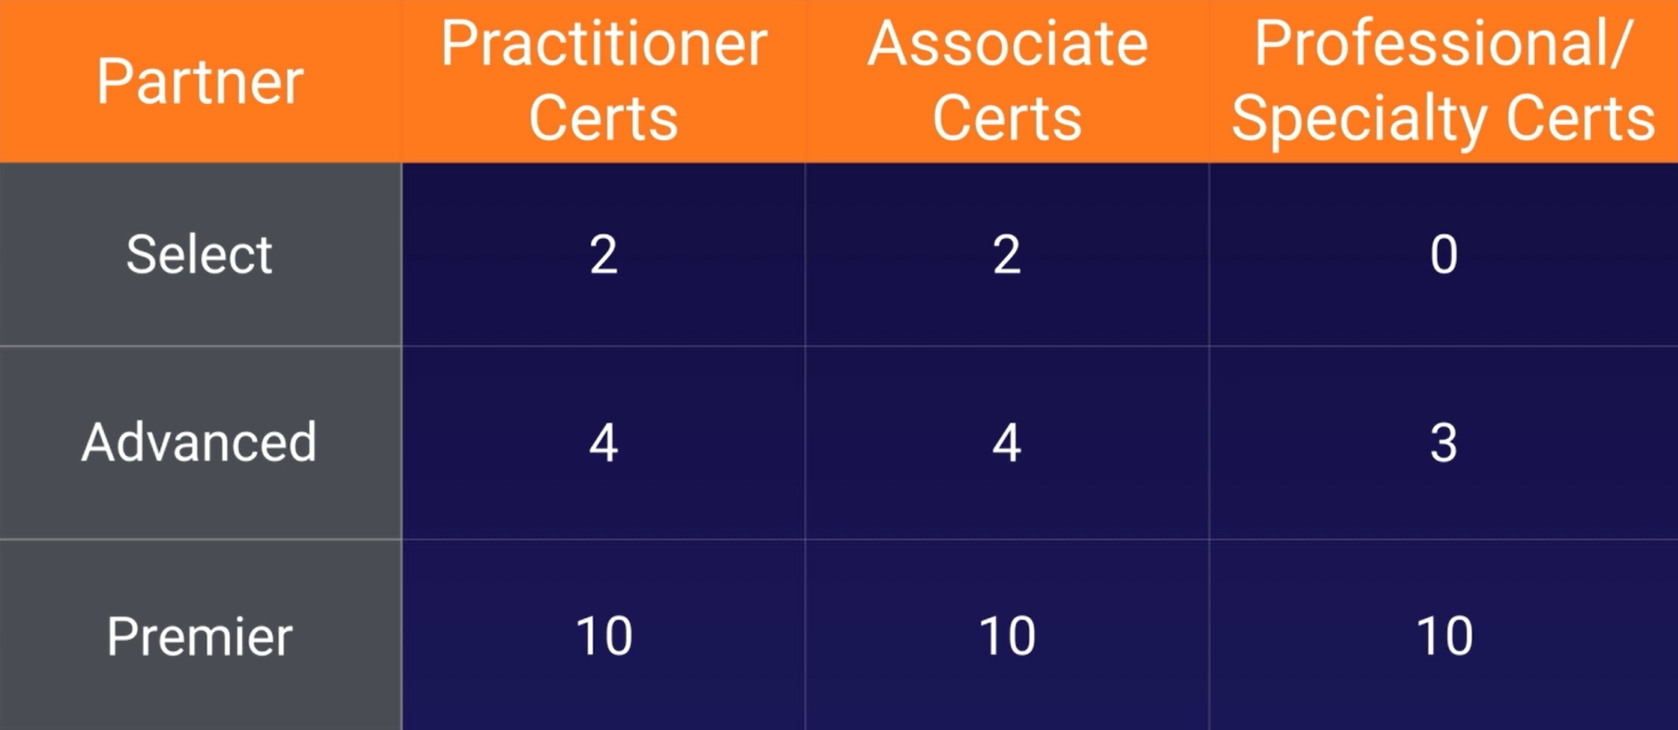
\includegraphics[width = 100mm]{./images/AWS-partner-tiers.png}
	\caption{AWS Partnership tiers and requirements are shown in the above image. Please look at the benefits at this \href{https://aws.amazon.com/blogs/apn/make-the-most-of-your-aws-partner-network-apn-benefits/}{[link]}.}
	\label{AWS-partner-tiers}
\end{figure}

\section{Amount of AWS Features and Services}
AWS is too vast. You should have broad overall knowledge, and then you should have your specialization. The number of services increase very fast:

\begin{enumerate}
	\item 2011: 82.
	\item 2015: 735.
	\item 2019: 2400.
\end{enumerate}

Hence, please keep learning.

Cloud spending is increasing very fast in the world. Software is eating the world and cloud is eating software.

AWS are leading cloud providers and are growing in public cloud market share at a rate extensively faster than their competitors. AWS makes up $51.8\%$ worldwide cloud market share. It is a safe industry due to it's hyper-growth.

